% !TeX spellcheck = en_GB
% Template for ICASSP-2010 paper; to be used with:
%          mlspconf.sty  - ICASSP/ICIP LaTeX style file adapted for MLSP, and
%          IEEEbib.bst - IEEE bibliography style file.
% --------------------------------------------------------------------------
\documentclass{article}
\usepackage{amsmath,graphicx,02460}
\usepackage{url}
\usepackage{mathtools}
\usepackage{booktabs}
\usepackage{caption}
\toappear{02456 Deep Learning, DTU Compute, Autumn 2019}
\newcommand{\pro}{\ensuremath{\ \%}}

% Example definitions.
% --------------------
\def\x{{\mathbf x}}
\def\L{{\cal L}}
\usepackage{fancyhdr}
\pagestyle{plain}

% Title.
% ------
\title{SegNet on Drone Images: Image Segmentation for Smart Agriculture}
%
% Single address.
% ---------------
\name{			Anders Henriksen, Asger Schultz, Oskar Wiese, 	Mads Andersen,
	Søren Winkel Holm }
\address{\{s183904, s183912, s183917, s173934, s183911\}@student.dtu.dk}
%
% For example:
% ------------
%\address{School\\
%	Department\\
%	Address}
%
% Two addresses (uncomment and modify for two-address case).
% ----------------------------------------------------------
%\twoauthors
%  {A. Author-one, B. Author-two\sthanks{Thanks to XYZ agency for funding.}}
%	{School A-B\\
%	Department A-B\\
%	Address A-B}
%  {C. Author-three, D. Author-four\sthanks{The fourth author performed the work
%	while at ...}}
%	{School C-D\\
%	Department C-D\\
%	Address C-D}
%
\begin{document}
%\ninept
%

\maketitle
%
\begin{abstract}
 Identifying crops, weeds and dirt in a typical field is a major task for a farmer. An image segmentation task, where the goal is to classify where in the field there are crops, weed and soil based on drone images of a field, can speed up and automate the time consuming task for a farmer. In this paper, we present an implementation of the deep network: SegNet and a strategy for training. The purpose is to build an efficient deep network: both memory wise and during inference. The architecture consists of an auto-encoder format, where the max-pooling indices are used as skip connections. Several advanced data augmentation techniques is used to train the network to classify crops, weed and soil in a drone image of a suger cane field in Colombia. In conclusion, the deep network is able to classify the crops, weed and soil and obtains a F1-score at $ 85 \% $. 
\end{abstract}
%
\begin{keywords}
One, two, three, four, five
\end{keywords}
%
\section{Introduction}
\label{sec:intro}

\subsection{Motivation}
Image segmentation and object classification have been a huge talking point in recent years. This is partly due to the wide array of possible applications and the recent interest in machine learning and, in particular, deep learning. One such important application is seperating weeds, crops and dirt in aerial drone images of a field. Applying the SegNet architecture to this field of crop segmentation could allow for smart agriculture that circumvents the many laborious man-hours of manual classification. Using SegNet for this classification could also prove useful in terms of the computational efficiency, as this allows for end-to-end training and makes embedded systems, e.g. in drones, feasible.

\subsection{Dataset and Preprocessing}
The primary dataset in question consists of two large, high resolution orthomosaic RGB images of a sugar cane field\footnote{Aerial image: http://www.lapix.ufsc.br/wp-content/uploads/2019/05\\/sugarcane2.png\\
Ground truth: http://www.lapix.ufsc.br/wp-content/uploads/2019/05\\/crop6GT.png}.
The first image consists of several drone images stitched together, with the second image of the same size being the manually labelled human ground truth, labelled by an expert biologist.
The three classes each have a corresponding colour -- crop rows are green, weeds are yellow, and soil is red.
Void pixels are black.

We also used second, smaller dataset from a corn field. \textbf{INSERT LINK}
We did not use this for hyperparameter optimization or architechtural decisions like this primary dataset.
Instead, only a train/test split was used to evaluate the network using the exact same hyperparameters.
We did not perform any hyperparameter optimization or architechtural decisions based on this dataset.
Instead, only a train/test split was used to evaluate the network using exact same hyperparameters.

\subsection{Motivation}
Image segmentation and object classification have been a huge talking point in recent years. This is partly due to the wide array of possible applications and the recent interest in machine learning and, in particular, deep learning. One such important application is seperating weeds, crops and dirt in aerial drone images of a field. Applying the SegNet architecture to this field of crop segmentation could allow for smart agriculture that circumvents the many laborious man-hours of manual classification. Using SegNet for this classification could also prove useful in terms of the computational efficiency, as this allows for end-to-end training and makes embedded systems, e.g. in drones, feasible.

\subsection{Goal and Application}


In the following segments of this paper, the relevant methods, results and discussion will be covered; In section 2, methods such as regularization, data augmentation, metrics and chosen loss function are described. The results are tabulated in section 3. Section 4 is a discussion of the results and accuracy of the reconstruction, a comparison to other similar methods as well as a perspective on the problem. The relevant references are included in section 5.

\section{METHODS}
\label{sec:format}

\subsection{Preprocessing and Data Augmentation}
In order to get the most out of the data, preprocessing is needed.
First, the RGB values of the non-void pixels of the aerial image are standardized, and a matrix is used to represent the ground truth.
Each entry corresponds to a pixel and contains a number 0-2 for the different classes or 3 for void.
The images are then padded with black pixels and cropped into smaller $ 512\times 512 $ pixel images.
Any of these images containing only black pixels are discarded, leaving a total of 108 pairs of aerial photo/ground truth images.
These are then split into 69 training, 18 validation, and 25 test images.

In order to increase the effective size of the dataset, we perform aggressive data augmentation.
When training the network, each pair of aerial photo/ground truth images is randomly cropped into $ 256\times 256 $ pixel images.
Furthermore, we applied a 50\pro\ chance of performing a top/down flip as well as a 50\pro\ chance of left/right flip to each image pair.
Even though data augmentation is not as a good as more independent data, it still allows the network to generalize better and overfit less.

The same preprocessing was applied to the secondary dataset with the only difference being that black pixels were a class, so these were not left out of the training and evaluation.
We ended up with \textbf{INSERT NUMBER OF IMAGES}

\subsection{Regularization}
Because deep neural networks are such highly flexible models, regularization is necessary on top of the data augmentation to further reduce overfitting.
This is done in two ways.

Dropout at 10\pro\ is used after each blue block in the network (see Fig. \ref{fig:arch}).
This randomly shuts off nodes during training leading to node redundancy and variability, as the same input will vary somewhat in its output, which learns the network to generalize better.
We experimented with higher dropout, but found that too much would significantly reduce learning.

Batch normalization is applied after each dropout.
This standardizes the activations, keeping them close to zero.
As a result, the weights and biases also stay close to zero, which reduces the flexibility of the model, leading to less overfitting.
Batch normalization also has several other benefits, such as reducing the vanishing gradient problem and allowing for a higher learning rate and thus faster convergence time. \cite{bn}
\\
\\
\subsection{}
The encoder part of the network creates a rich feature map representing the image content. The more 
layers of max-pooling there are the more translation invariance for robust 
classification can be achieved. The boundary detail is very important when 
dealing with image segmentation. Hence, capturing boundary information in 
the feature maps of the encoder before upsampling is important. This can 
simply be done by storing the whole feature map, but due to memory 
constrains only the maxpooling indices are saved, which is a good 
approximation of the feature maps. 
\subsection{Training: Learning from Quality over Quantity}
For training, finding the optimal weights of the network, the widely used Adam optimizer  was implemented because the addition of momentum to the efficient and effective Stochatic Gradient Descent algorithm is shown to giver faster convergence in a wide range of computer vision tasks \cite{Adam}. The training was done in 3000 epochs each consisting of mini batches of size 3.

A more interesting choice was the loss function. It was clear that 3-class cross entropy should be used as this function, for a Softmax network such as SegNet, can be seen as the following the maximum likelihood principle and implementing minus log likelihood loss. The direct implementation of this, however, failed to consider a deep issue in Image Segmentation which had considerable effect on this limited data set: \textit{class imbalance}. 
In this data set, there is \(\sim 93 \%\) pixels belonging to the \textit{dirt}-class which arguably is the least interesting and initial tests saw the network behave too much as a baseline; simple features in early layers which classified almost everything as dirt were not penalized enough and learning was not stable. 

As resampling an image data set is computationally expensive and it was desired that the network learned to focus on important pixels, it was chosen the main training experiment of this report should use \textit{weighted cross entropy} where each class is weighted by \(1-\nu\); where \(\nu\) is its frequency thus focusing more on the classes crops and weeds than in the vanilla cross entropy. The implemented loss of \(N\) pixels in a one-hot encoded \((N \times  3)\) output matrix \(\mathbf X^\text{pred}\) with the true classes \(\mathbf c\) was then:
\[
L = \underbrace{
	\vphantom{\sum_{i}}
	\frac 1 N
	\sum_{\mathclap {i=1}}^{N}
}
_{\mathllap{\text{Mean over minibatch}}}
\underbrace{ 
	\vphantom{\sum_{i}}
	\mathbf{w}[i, c_i]}
_{\mathclap{\text{Class weight}}}  
\cdot 
\underbrace{
	\log 
	\frac
	{-\exp\mathbf X^\text{pred}[i, c_i]}
	{\sum_{j=1}^{3}\exp\mathbf X^\text{pred}[i, j]}
}_{\mathclap{\text{3-class cross entropy}}}
\] 
To test the importance of this frequency balancing for this data set, another training experiment was set up without weighting of the cross entropy loss.
\subsection{Evaluation Metrics: Finding the Important Story}
In the compared image segmentation literature no single accuracy measure can be described  as the canonical metric resulting in a number of metrics being compared \cite{eval, Metric}.  A collection of different metrics are usable as the performance difference on global and local scale is relevant. 
%	\item Different metrics important in different fields.
Four simple accuracy measures are used here to mirror the SegNet paper \cite{seg} though more complex measures which fit better with human evaluation exist \cite{eval}. 

The simple global accuracy, the frequency of correct classifications, is not the most meaningful measure for class imbalanced data sets such as this (where the baseline achieves \(>90\%\)) but is in the literature noted to be important for a smooth classification \cite{seg}. Another simple measure is the mean of the accuracies of model on the three classes. This measure is still a naïve accuracy measure but is the metric which is being optimized for in the weighted cross entropy loss. 

The metric which is being seen as the main performance metric is the F1-score: The harmonic mean of precision of recall. This is used for comparison to other groups with same project and because this metric penalizes false positives and gives less credit to true negatives thus being better for unbalanced classes \cite{Metric}. A related score is the Mean Intersect over Union (MIoU), also known as the Jaccard Index, which penalizes false positives harder and is found to be better correlated to human evaluation though only \(\sim 0.5\) \cite{eval}. 

Both F1 and MIoU are calculated for each of the three classes and are then averaged to get the final score. Both of them favour region smoothness higher than boundary accuracy compared to semantic accuracy measures such as the Berkeley contour matching score \cite{seg}.

To estimate generalization performance, the models are compared by their performance on the \textit{test data set} which is kept separate from the training and validation data and is pre-divided for both data sets consisting of approximately \( 20\%\) of the images.  It is noted that this simple hold out evaluation method does not claim to give an accurate estimate of generalization error on \textit{any} data set but can statistically only be seen as an evaluation of the performance on the used data sets. 

\subsection{Experiments and Reconstruction}
When training the network, we used the following hyperparameters: Batch size of 3, dropout of 10\pro, and a learning rate of $ 1.5\cdot 10^{-4} $ with the ADAM optimization algorithm.
For the convolutional layers, kernel size was set to $ 3\times 3 $ and stride to $ 1 $, as deeper network structures tend to learn to better and faster with smaller kernels.
This is because the receptive field is the same as larger kernels in shallower networks, but the multiple layers allow for learning more complex structures.
In the encoder part, the first convolutional layer increased the number of channels to 64.
Thereafter, the first convolutional layer in each block doubled the number of channels, ending at 512.
In the max pooling layers, we used a $ 2\times 2 $ with a stride of 2, cutting the size of the feature maps to a quarter each time.
The decoder part exactly mirrored this structure.

The training can be recreated using the Jupyter Notebook at \texttt{src/image-segmentation.ipynb} folder in the Github repository.
Because training the network takes close to 30 GB of VRAM, we have implemented a simpler version of SegNet with fewer layers that takes significantly less memory to train.
This is controlled using the \texttt{use\_simple} variable, which is set to \texttt{True} by default.


\subsection{Unification of Cropped Image Predictions}
In a real-world application of the field classification a farmer would want a complete and precise segmentation of his whole field at once, such that fertilizer and pesticides can be distributed accordingly. To accomplish this, a reconstruction of the smaller image inferences is neccesary. The most straight forward method of combining the smaller images, by simply lining them up next to each other results in a very rough transition between the smaller inferences. This can be seen in the left side of figure \ref{fig:earlylatereconstruction}. The blocky nature of the field prediction is caused by a lack of information from neighbouring pixel when inference is performed near the borders of an image. To solve this problem, we have chosen to increase the size of the cropped images and add some overlap, and then infer on these enlarged pictured. In the procedure of joining the enlarged cropped pictures they are cropped again, to avoid the border areas. At the cost of computational efficiency more information is available near the borders and a smooth transition between the smaller inferences can be achieved. This can be seen in the right side of figure \ref{fig:earlylatereconstruction}. A visualization of the reconstruction technique can be seen in appendix \ref{reconstruction_technique}.



\begin{figure}
	\centering
	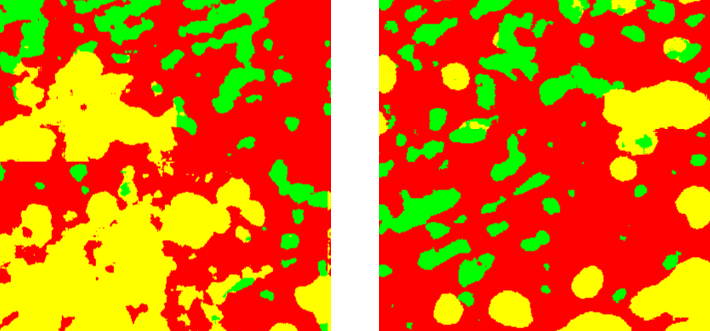
\includegraphics[width=0.9\linewidth]{early_late_reconstruction2}
	\caption{\textbf{Left:} Smaller inferences put next to eachother without use of reconstruction techniques. \textbf{Right:} Reconstruction with padding and overlap between smaller inferences.}
	\label{fig:earlylatereconstruction}
\end{figure}





\section{RESULTS}
\label{sec:illust}

\begin{table}[!htb]
	\centering
	\begin{tabular}{l r r r r}
		\textbf{Train results} & & & & \\
		\toprule
		Method  &  G.acc.  &  C.acc.  &  Mean IoU  &  F1 \\ \midrule
		Baseline  &  0.91  &  0.33  &  n/a  &  0.32 \\
		\textbf{Standard}  &  0.97  &  0.90  &  0.80  &  0.88 \\
		Simple loss   &  0.96  &  0.71  &  0.66  &  0.78 \\
		\midrule 
		Corn Baseline  &  0.39  &  0.33  &  0.13  &  0.19 \\
		Corn Results  &  0.79  &  0.78  &  0.65  &  0.79 \\
		\bottomrule
	\end{tabular}
\end{table}

\begin{table}[!htb]
	\centering
	\begin{tabular}{l r r r r}
		\textbf{Test results} & & & & \\
		\toprule
		Method  &  G.acc.  &  C.acc.  &  Mean IoU  &  F1 \\ \midrule
		Baseline  &  0.94  &  0.33  &  n/a  &  0.32 \\
		\textbf{Standard}  &  0.98  &  0.86  &  0.75  & \textbf{ 0.85} \\
		Simple loss  &  0.97  &  0.61  &  0.57  &  0.69 \\
		\midrule
		USC SegNet  &  n/a  &  n/a  &  0.79  &  0.96 \\
		USC UNet  &  n/a  &  n/a  &  0.75  &  0.93 \\
		Cellari DNN  &  n/a  &  n/a  &  n/a  &  0.88 \\
		\midrule 
		Corn Baseline  &  0.32  &  0.33  &  0.11  &  0.16 \\
		Corn Results  &  0.35  &  0.36  &  0.21  &  0.34 \\
		\bottomrule
	\end{tabular}
\end{table}
\noindent Above, the G.acc. refers to global accuracy, C.acc to class accuracy and B.F1 to the F1-score.
USC is the first work on the data set \cite{brazil} and Cellari is the work from the procet supervisor \url{cellari.io}.
Note that we don't have access for full results for other implementations and, importantly, that the USC. implementations do not have the same train/test-split as the one used for this project.
\begin{figure}[!htb]
	\centering
	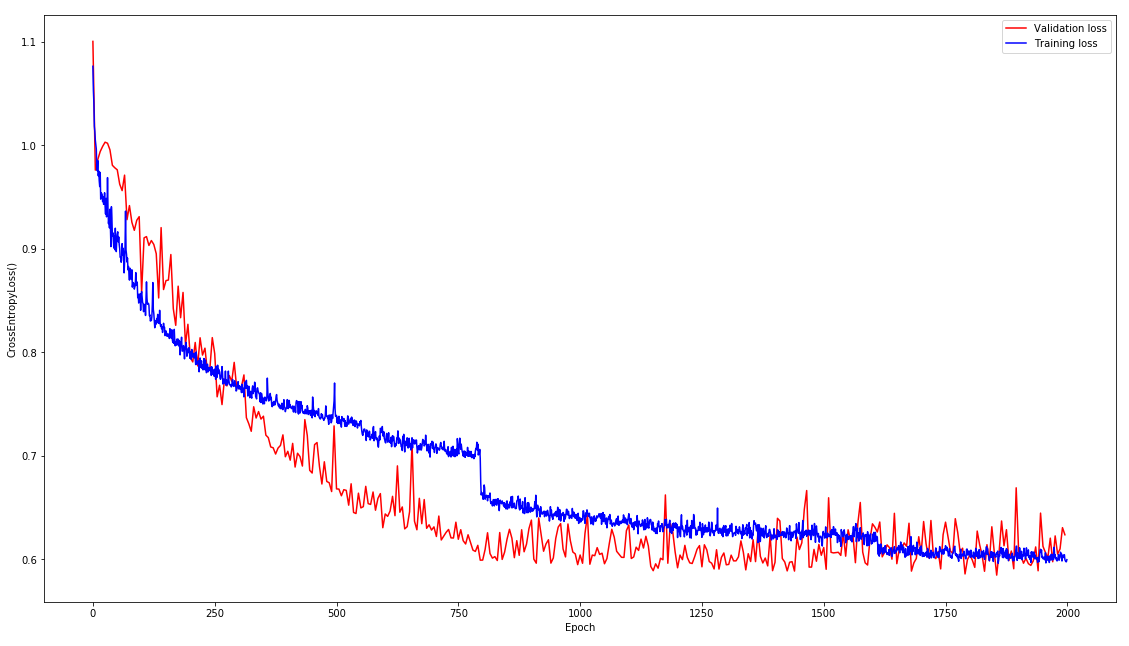
\includegraphics[width=0.9\linewidth]{../../poster/loss}
	\caption{}
	\label{fig:loss}
\end{figure}


% STANDARD BASELINE, CELLARIO AND COMPARED RESULTS LIGGER STADIG I POSTER

%STANDARD

%2019-12-10 22:31:52.335662	Calculating train accuracy measures...
%2019-12-10 22:32:04.165629	Accuracy measures: Global acc.: 0.9706
%Class acc.: 0.8993
%Mean IoU.: 0.7967
%Bound. F1: 0.8818
%
%2019-12-10 22:32:04.167743	Calculating test accuracy measures...
%2019-12-10 22:32:08.005059	Test accuracy measures: Global acc.: 0.9768
%Class acc.: 0.8585
%Mean IoU.: 0.7541
%Bound. F1: 0.851

%SIMPLELOSS
%2019-12-11 01:20:01.124762	Calculating train accuracy measures...
%2019-12-11 01:20:12.598002	Accuracy measures: Global acc.: 0.957
%Class acc.: 0.7078
%Mean IoU.: 0.6629
%Bound. F1: 0.7789
%
%2019-12-11 01:20:12.599878	Calculating test accuracy measures...
%2019-12-11 01:20:16.252676	Test accuracy measures: Global acc.: 0.9653
%Class acc.: 0.6107
%Mean IoU.: 0.5737
%Bound. F1: 0.6922


%CORN BASELINE 
%2019-12-28 16:30:59.018404	Evaluating Baseline

%2019-12-28 16:31:05.300109	Training accuracy measures: Global %acc.: 0.3925
%Class acc.: 0.3333
%Mean IoU.: 0.1308
%Bound. F1: 0.1879

%2019-12-28 16:31:06.241630	Test accuracy measures: Global %acc.: 0.3193
%Class acc.: 0.3333
%Mean IoU.: 0.1064
%Bound. F1: 0.1613


%CORN RESULTS

%2019-12-28 18:57:27.694899	Accuracy measures: Global acc.: 0.7938
%Class acc.: 0.7819
%Mean IoU.: 0.6505
%Bound. F1: 0.7877
%

%2019-12-28 18:57:28.459897	Test accuracy measures: Global acc.: 0.3518
%Class acc.: 0.3556
%Mean IoU.: 0.2069
%Bound. F1: 0.3398


\section{DISCUSSION}

\subsection{Performance of Networks: Loss and Size matter}
The main performance benchmark for this test of the SegNet implementation is the test F1-score on the Brazil sugar cane data set: \textbf{85\%}.
This score is seen as acceptable as it reaches a score which generally seen as high for image segmentation where human agreement of segmentation is often limited \cite{eval}.  It also clearly outperforms the baseline score of 0.32\% but fails to reach the performance of other Deep Neural Networks: The Cellari DNN and the Universidad de Catarina implementations are 3-11 \% points higher. 

These differences can be due to data augmentation practises and hyper parameter optimization as the hyper parameters for these implementations could not be accessed.
For data augmentation, this project chose to use flipping and random cropping heavily and the forceful croppings from 512x512 to 350x350 (halving the number of pixels) might have limited the learning of the model as less data was accessible for each parameter update. 

The motivation for this data augmentation choice was mainly because of computational limits in training but it also resulted in no discernable trace of overfitting as can be seen from figure \eqref{fig:loss} and the minor differences in train and the limited differences in test and train results.

This indicates that controlling the size of random croppings is another regularization parameter usable for balancing the bias/variance-tradeoff of image segmentation tasks.
 
For MIoU, the measure which is closest linked with human evaluation \cite{eval}, the differences between this reports main network and the other implementations more slight. 
\\
\\
The test of the \textbf{loss function} gives clear results: The difference of 0.16 in test F1 score is assumed to be significant and the results for the unweighted cross entropy loss functions seem to fit the expected:
There is virtually no difference in the global accuracy -- for which the simple loss function optimizes -- showing that learning has occurred.
The large differences in the class-balanced accuracy measures indicate that, when all classes are of importance, the frequency weighted cross entropy loss should be used  for unbalanced data.
\\
\\
The test of the small, novel \textbf{corn field data} set gives disappointing results: Only a 

\label{sec:foot}
\subsection{Comparison of Different Image Segmentation Neural Networks}
\begin{itemize}
	\item Several competing network structures with high performance in image segmentation. U-net, FCN, DeepLabv1, DeconvNet
	\item Purpose of SegNet, efficient
	\item 3 out of the 4 mentioned uses the encoder from the famous VGG16 paper, but differ in decoder.
	\item FCN, No decoder -> Blocky segmentation, but very efficient in inference time.
	\item DeconvNet, Deconvolution and fully connected layers. 
	\item U-Net, (different purpose), skip connections. 
	\item Main takeaway  
	\item (Deeplabv-LargeFOV \& FCN)
\end{itemize}
	
\subsubsection{Leading architectures in the image segmentation field}
In the field of image segmentation there are several different neural network architectures that excel in different types of problems. Among the most acknowledged architectures are U-net, DeepLabv1, DeconvNet and FCN. 
All of these networks differ in several ways and it is important to emphasize that each network is designed to excel in a specific branch of image segmentation. U-net is as an example designed for medical image segmentation, whereas SegNet is designed such that it can be used in embedded systems. Each branch of problems has its own challenges and limitations. Therefore it is necessary to apply problem-specific methods to optimally segment the images. 
As mentioned earlier the purpose of SegNet is to be efficient in inference time and memory-wise, such that it can be used in embedded systems. And these two aspects are the ones we are interested in comparing SegNet and the other architectures. 
SegNet and its competitors have a quite similar performance in terms of accuracy on both road map scenes and the benchmark dataset known as SUN RGB-D, which is an indoor scene segmentation challenge \cite{seg}. 
With respect to the architecture of the encoder of the competing networks, SegNet and three of the four competitors (FCN, DeconvNet, U-net) have an almost topologically identical encoder as the one from the well known VGG16 network. One important difference between SegNet and the three others is that SegNet is without the final fully connected layers, which decreases the amount of trainable parameters with almost 90\% \cite{seg}. 
All of the networks differ in decoding structure and techniques that is applied, and as a common denominator for FCN, DeconvNet and DeepLab-LargeFov are nearly twice as much memory during inference used. Among the heavy users of memory are the fully connected layers of the DeconvNet and FCN, and the skip connections in the U-Net. In comparrison with the same 3 structures does SegNet come in second only bested by DeepLab-LargeFOV with respect to inference time.


The encoder part of the network has only 14.7 million parameters compared to partially fully connected structures that tend to have well over 100 million. \cite{seg}


\subsection{Potential in SegNet}
The architecture of SegNet allows for an easy and fast end to end training of the network. As a consequence of this SegNet is easily modified into other use cases without much technical effort. Because of the low memory usage and the speed of which the inference takes place SegNet could prove to be a good choice for self-driving cars and drones. However, it can be challenging and costful to acquire labelled data as this typically involves professionals manually doing the labelling. In our project we only have a single field image, which is probably not representative of similar fields under different circumstances such as lighting, type of crop and season. (The robustness of our network has been tested by running inference on a different data set and with XXX result (EKSILD DATA?)  The robustness of the network can be enhances by different augmentation techniques that is problem dependant. There exits a vast amount of different techniques and some have proved useful in medical imaging, whereas other are preferred in other problem settings. \cite{seg}

\subsection{Extension of network}


\subsection{Conclusion}


 
\subsection{Summary}
The purpose of this project has been build an efficient neural network architecture for semantic pixel-wise segmentation on a crop field. The neural network has to be efficient especially in terms of memory usage and time during inference, such that it can be used in embedded system such as drones are cars. The architecture implemented goes under the name SegNet \ref{SEGNETREFERENCE}, and it consists of an encoder and a corresponding decoder network and ends with a pixelwise classification layer. The purpose of the encoder is to reduce the dimensionallity and extracts the useful information in the image thereby creating a dense feature maps that can be classified. This procedure is performed by using blocks of convolutional layers, each block ending with a max pooling layer. The decoder has to upsample the low-resolution feature map back into full input resolution, such that a precise pixelwise classification can take place. During the encoding procedure only the most characteristic (Replace with another term) information is extracted with max pooling layers, and local information is lost . This local information is neccesary for a precise classification and therefor SegNet uses max-pooling indices as skip connections to retain this local information. During the upsampling these max pooling indices are used to create a sparse feature map and afterwards convolutional layers are use to create more dense feature maps. The use of max pooling indices are a very efficient way of storing local information with only a slight loss of accuracy. Our results show that ------xx----. Conclusion ----x----.


\bibliographystyle{IEEEbib}
\bibliography{refs}
\subsection{Appendix}
\begin{figure}[h!]
	\centering
	\includegraphics[width=0.7\linewidth]{"reconstruction DL"}
	\caption{Reconstruction of the smaller inferences into a unified field prediction.}
	\label{reconstruction_technique}
\end{figure}



\end{document}
% !TeX spellcheck = en_GB
% Template for ICASSP-2010 paper; to be used with:
%          mlspconf.sty  - ICASSP/ICIP LaTeX style file adapted for MLSP, and
%          IEEEbib.bst - IEEE bibliography style file.
% --------------------------------------------------------------------------
\documentclass{article}
\usepackage{amsmath,graphicx,02460}
\usepackage{url}
\usepackage{mathtools}
\toappear{02456 Deep Learning, DTU Compute, Autumn 2019}
\newcommand{\pro}{\ensuremath{\ \%}}

% Example definitions.
% --------------------
\def\x{{\mathbf x}}
\def\L{{\cal L}}

% Title.
% ------
\title{SegNet on Drone Images: Image Segmentation for Smart Agriculture}
%
% Single address.
% ---------------
\name{			Anders Henriksen, Asger Schultz, Oskar Wiese, 	Mads Andersen,
	Søren Winkel Holm }
\address{\{s183904, s183912, s183917, s173934, s183911\}@student.dtu.dk}
%
% For example:
% ------------
%\address{School\\
%	Department\\
%	Address}
%
% Two addresses (uncomment and modify for two-address case).
% ----------------------------------------------------------
%\twoauthors
%  {A. Author-one, B. Author-two\sthanks{Thanks to XYZ agency for funding.}}
%	{School A-B\\
%	Department A-B\\
%	Address A-B}
%  {C. Author-three, D. Author-four\sthanks{The fourth author performed the work
%	while at ...}}
%	{School C-D\\
%	Department C-D\\
%	Address C-D}
%
\begin{document}
%\ninept
%

\maketitle
%
\begin{abstract}
Identifying crops, weeds and dirt in a typical field is a major task for a farmer. An image segmentation task, where the goal is to classify where in the field there are crops, weed and soil based on drone images of a field, can speed up and automate the time consuming task for a farmer. In this paper, we present an implementation of the deep network: SegNet and a strategy for training. The purpose is to build an efficient deep network: both memory wise and during inference. The architecture consists of an auto-encoder format, where the max-pooling indices are used as skip connections. Several advanced data augmentation techniques is used to train the network to classify crops, weed and soil in a drone image of a suger cane field in Colombia. In conclusion, the deep network is able to classify the crops, weed and soil and obtains a harmonic mean of precision and recall at $ 84 \% $.
\end{abstract}
%
\begin{keywords}
Deep Network, Image Segmentation, Ground Truth Segmentation, SegNet, Data Augmentation
\end{keywords}
%
\section{Introduction}
\label{sec:intro}

\subsection{Dataset and Preprocessing}
Our primary dataset consists of two large, high resolution orthomosaic RGB images of a sugar cane field\footnote{Aerial image: http://www.lapix.ufsc.br/wp-content/uploads/2019/05\\/sugarcane2.png\\
Ground truth: http://www.lapix.ufsc.br/wp-content/uploads/2019/05\\/crop6GT.png}.
The first image consists of several drone images stitched together, with the second image of the same size being the by an expert biologist manually labelled human ground truth.
The three classes each have a corresponding colour -- crop rows are green, weeds are yellow, and soil is red.
Void pixels are black.

We also used second, smaller dataset from a corn field. \textbf{INSERT LINK}
We did not use this for hyperparameter optimization or architechtural decisions like this primary dataset.
Instead, only a train/test split was used to evaluate the network using exact same hyperparameters.

\subsection{Motivation}
Image segmentation and object classification have been a huge talking point in recent years. This is partly due to the wide array of possible applications and the recent interest in machine learning and, in particular, deep learning. One such important application is seperating weeds, crops and dirt in aerial drone images of a field. Applying the SegNet architecture to this field of crop segmentation could allow for smart agriculture that circumvents the many laborious man-hours of manual classification. Using SegNet for this classification could also prove useful in terms of the computational efficiency, as this allows for end-to-end training and makes embedded systems, e.g. in drones, feasible.

\subsection{Goal and Application}


In the following segments of this paper, the relevant methods, results and discussion will be covered; In section 2, methods such as regularization, data augmentation, metrics and chosen loss function are described. The results are tabulated in section 3. Section 4 is a discussion of the results and accuracy of the reconstruction, a comparison to other similar methods as well as a perspective on the problem. The relevant references are included in section 5.

\section{METHODS}
\label{sec:format}

\subsection{Preprocessing and Data Augmentation}
In order to get the most out of the data, preprocessing is needed.
First, the RGB values of the non-void pixels of the aerial image are standardized, and a matrix is used to represent the ground truth.
Each entry corresponds to a pixel and contains a number 0-2 for the different classes or 3 for void.
The images are then padded with black pixels and cropped into smaller $ 512\times 512 $ pixel images.
Any of these images containing only black pixels are discarded, leaving a total of 108 pairs of aerial photo/ground truth images.
These are then split into 69 training, 18 validation, and 25 test images.

In order to increase the effective size of the dataset, we perform aggressive data augmentation.
When training the network, each pair of aerial photo/ground truth images is randomly cropped into $ 256\times 256 $ pixel images.
Furthermore, we applied a 50\pro\ chance of performing a top/down flip as well as a 50\pro\ chance of left/right flip to each image pair.
Even though data augmentation is not as a good as more independent data, it still allows the network to generalize better and overfit less.

The same preprocessing was applied to the secondary dataset with the only difference being that black pixels were a class, so these were not left out of the training and evaluation.
We ended up with \textbf{INSERT NUMBER OF IMAGES}

\subsection{The Model}

\subsubsection*{SegNet}
%
The SegNet model architecture utilizes convolutional neural networks (CNN). CNN's work by convolving over an image with a kernel. The kernel size, stride and padding are all adjustable parameters that help to fit the kernel to a specific image dimension or keep the dimensions of the image constant. 
%Encoder / Decoder  
SegNet's model architecture has an encoder-decoder structure. The encoder create dense feature maps which allow for translational invariance, and the decoder learns to seperate the classes. The model consists of a total of ten blocks which either have two or three convolutional layers. Encoder blocks ends with a max-pooling layer whereas decoder blocks starts with an un-pooling layer. Every encoder and decoder block has applied dropout to prevent overfitting, batchnorm for normalization, ReLU for non-linearity and max-pool for translational invariance. The last layer is a softmax layer, which allows an evaluation of the prediction of the model. The dimensions of the encoder and decoder blocks are equal and mirrored. Thus, the dimension of the input and output are the same. \\
%Skip connections 
 The encoder part of the network creates a rich feature map representing the image content. The boundary detail is very important when dealing with image segmentation. Hence, apprehending boundary information in the feature maps of the encoder before upsampling is important. This can simply be done by storing the whole feature map, but will be very memory inefficient. Therefore, skip connections between each encoder and decoder block are introduced by storing only the max-pooling indices from each max-pooling layer. Its been shown in the literature, that storing the max pooling indices is a good approximation of the actual feature map \cite{seg}. 




\subsection{Regularization}
Because deep neural networks are such highly flexible models, regularization is necessary on top of the data augmentation to further reduce overfitting.
This is done in the following two ways.

Dropout at 10\pro\ is used after each blue block in the network (see Fig. \ref{fig:arch}).
This randomly shuts off nodes during training leading to node redundancy and variability, as the same input will vary somewhat in its output, which learns the network to generalize better.
We experimented with higher dropout, but found that too much would significantly reduce learning.

Batch normalization is applied after each dropout.
This standardizes the activations, keeping them close to zero.
As a result, the weights and biases also stay close to zero, which reduces the flexibility of the model, leading to less overfitting.
Batch normalization also has several other benefits, such as reducing the vanishing gradient problem and allowing for a higher learning rate and thus faster convergence time. \cite{bn}
\\

\subsection{Loss Function: Quality over Quantity}
Multi-class cross entropy because:
\begin{itemize}
	\item Softmax Network: Minus log likelihood
	\item Can be seen as a classic multiclass classifier -- just on a pixel-by-pixel basis.
\end{itemize}
Weighted cross entropy because:
\begin{itemize}
	\item Unbalanced class distribution: Network has to learn to focus on important pixels: Don't classify everything as dirt.
	\item Initial tests made the network behave as the baseline: Simple features in early layers got were not penalized enough and learning was not stable.
	\item Resampling expensive
\end{itemize}
\subsection{Metrics}
Had to use different metrics because
\begin{itemize}
	\item Not agreement in Image Segmentation papers.
	\item Want to get accuracy on a global scale and on a class scale.
	\item Different metrics important in different fields.
\end{itemize}
The metrics \footnote{https://hal.inria.fr/hal-01581525/document}\footnote{
	http://www.bmva.org/bmvc/2013/Papers/paper0032/paper0032.pdf} 
\begin{itemize}
	\item Global accuracy: Trivial and  not very important because of class imbalance but is good for smoothness
	\item Mean class-wise accuracy: Takes class imbalance into account. Is what is being optimized for in the model.
	\item Mean Intersect over Union: "Jaccard Index".  Found to be better correlated with human classification though still only \(\approx 0.5\). Favours region smoothness highly and not boundary accuracy.
	\item Harmonic mean of precision and recall. To compare to others with same project. Penalizes false positives and gives less credit to true negatives thus being better for unbalanced classes.
\end{itemize}

\subsection{}
The encoder part of the network creates a rich feature map representing the image content. The more 
layers of max-pooling there are the more translation invariance for robust 
classification can be achieved. The boundary detail is very important when 
dealing with image segmentation. Hence, capturing boundary information in 
the feature maps of the encoder before upsampling is important. This can 
simply be done by storing the whole feature map, but due to memory 
constrains only the maxpooling indices are saved, which is a good 
approximation of the feature maps. 
\subsection{Training: Learning from Quality over Quantity}
For training, finding the optimal weights of the network, the widely used Adam optimizer  was implemented because the addition of momentum to the efficient and effective Stochatic Gradient Descent algorithm is shown to giver faster convergence in a wide range of computer vision tasks \cite{Adam}. The training was done in 3000 epochs each consisting of mini batches of size 3.

A more interesting choice was the loss function. It was clear that 3-class cross entropy should be used as this function, for a Softmax network such as SegNet, can be seen as the following the maximum likelihood principle and implementing minus log likelihood loss. The direct implementation of this, however, failed to consider a deep issue in Image Segmentation which had considerable effect on this limited data set: \textit{class imbalance}. 
In this data set, there is \(\sim 93 \%\) pixels belonging to the \textit{dirt}-class which arguably is the least interesting and initial tests saw the network behave too much as a baseline; simple features in early layers which classified almost everything as dirt were not penalized enough and learning was not stable. 

As resampling an image data set is computationally expensive and it was desired that the network learned to focus on important pixels, it was chosen the main training experiment of this report should use \textit{weighted cross entropy} where each class is weighted by \(1-\nu\); where \(\nu\) is its frequency thus focusing more on the classes crops and weeds than in the vanilla cross entropy. The implemented loss of \(N\) pixels in a one-hot encoded \((N \times  3)\) output matrix \(\mathbf X^\text{pred}\) with the true classes \(\mathbf c\) was then:
\[
L = \underbrace{
	\vphantom{\sum_{i}}
	\frac 1 N
	\sum_{\mathclap {i=1}}^{N}
}
_{\mathllap{\text{Mean over minibatch}}}
\underbrace{ 
	\vphantom{\sum_{i}}
	\mathbf{w}[i, c_i]}
_{\mathclap{\text{Class weight}}}  
\cdot 
\underbrace{
	\log 
	\frac
	{-\exp\mathbf X^\text{pred}[i, c_i]}
	{\sum_{j=1}^{3}\exp\mathbf X^\text{pred}[i, j]}
}_{\mathclap{\text{3-class cross entropy}}}
\] 
To test the importance of this frequency balancing for this data set, another training experiment was set up without weighting of the cross entropy loss.
\subsection{Evaluation Metrics: Finding the Important Story}
In the compared image segmentation literature no single accuracy measure can be described  as the canonical metric resulting in a number of metrics being compared \cite{eval, Metric}.  A collection of different metrics are usable as the performance difference on global and local scale is relevant. 
%	\item Different metrics important in different fields.
Four simple accuracy measures are used here to mirror the SegNet paper \cite{seg} though more complex measures which fit better with human evaluation exist \cite{eval}. 

The simple global accuracy, the frequency of correct classifications, is not the most meaningful measure for class imbalanced data sets such as this (where the baseline achieves \(>90\%\)) but is in the literature noted to be important for a smooth classification \cite{seg}. Another simple measure is the mean of the accuracies of model on the three classes. This measure is still a naïve accuracy measure but is the metric which is being optimized for in the weighted cross entropy loss. 

The metric which is being seen as the main performance metric is the F1-score: The harmonic mean of precision of recall. This is used for comparison to other groups with same project and because this metric penalizes false positives and gives less credit to true negatives thus being better for unbalanced classes \cite{Metric}. A related score is the Mean Intersect over Union (MIoU), also known as the Jaccard Index, which penalizes false positives harder and is found to be better correlated to human evaluation though only \(\sim 0.5\) \cite{eval}. 

Both F1 and MIoU are calculated for each of the three classes and are then averaged to get the final score. Both of them favour region smoothness higher than boundary accuracy compared to semantic accuracy measures such as the Berkeley contour matching score \cite{seg}.

To estimate generalization performance, the models are compared by their performance on the \textit{test data set} which is kept separate from the training and validation data and is pre-divided for both data sets consisting of approximately \( 20\%\) of the images.  It is noted that this simple hold out evaluation method does not claim to give an accurate estimate of generalization error on \textit{any} data set but can statistically only be seen as an evaluation of the performance on the used data sets. 

\subsection{Experiments and Reconstruction}
When training the network, we used the following hyperparameters: Batch size of 3, dropout of 10\pro, and a learning rate of $ 1.5\cdot 10^{-4} $ with the ADAM optimization algorithm.
For the convolutional layers, kernel size was set to $ 3\times 3 $ and stride to $ 1 $, as deeper network structures tend to learn to better and faster with smaller kernels.
This is because the receptive field is the same as larger kernels in shallower networks, but the multiple layers allow for learning more complex structures.
In the encoder part, the first convolutional layer increased the number of channels to 64.
Thereafter, the first convolutional layer in each block doubled the number of channels, ending at 512.
In the max pooling layers, we used a $ 2\times 2 $ with a stride of 2, cutting the size of the feature maps to a quarter each time.
The decoder part exactly mirrored this structure.

The training can be recreated using the Jupyter Notebook in the \texttt{src} folder in the Github repository.
Because training the network takes close to 30 GB of VRAM, we have implemented a simpler version of SegNet with fewer layers that takes significantly less memory to train.
This is controlled using the \texttt{use\_simple} variable, which is set to \texttt{True} by default.


\subsection{Unification of Cropped Image Predictions}
In a real-world application of the field classification a farmer would want a complete and precise segmentation of his whole field at once, such that fertilizer and pesticides can be distributed accordingly. To accomplish this, a reconstruction of the smaller image inferences is neccesary. The most straight forward method of combining the smaller images, by simply lining them up next to each other results in a very rough transition between the smaller inferences. This can be seen in the left side of figure \ref{fig:earlylatereconstruction}. The blocky nature of the field prediction is caused by a lack of information from neighbouring pixel when inference is performed near the borders of an image. To solve this problem, we have chosen to increase the size of the cropped images and add some overlap, and then infer on these enlarged pictured. In the procedure of joining the enlarged cropped pictures they are cropped again, to avoid the border areas. At the cost of computational efficiency more information is available near the borders and a smooth transition between the smaller inferences can be achieved. This can be seen in the right side of figure \ref{fig:earlylatereconstruction}. A visualization of the reconstruction technique can be seen in appendix \ref{reconstruction_technique}.



\begin{figure}
	\centering
	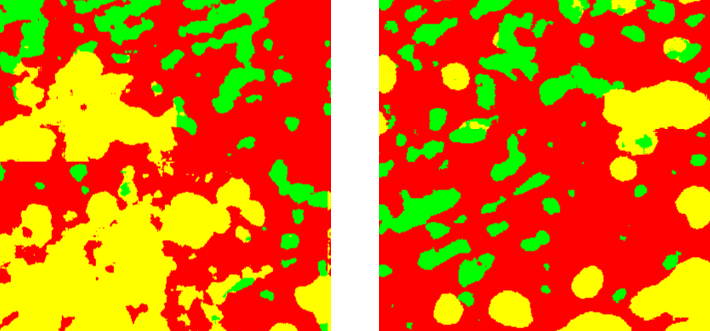
\includegraphics[width=0.9\linewidth]{early_late_reconstruction2}
	\caption{\textbf{Left:} Smaller inferences put next to each other without use of reconstruction techniques. \textbf{Right:} Reconstruction with padding and overlap between smaller inferences.}
	\label{fig:earlylatereconstruction}
\end{figure}





\section{RESULTS}
\label{sec:illust}
% STANDARD BASELINE, CELLARIO AND COMPARED RESULTS LIGGER STADIG I POSTER

%STANDARD

%2019-12-10 22:31:52.335662	Calculating train accuracy measures...
%2019-12-10 22:32:04.165629	Accuracy measures: Global acc.: 0.9706
%Class acc.: 0.8993
%Mean IoU.: 0.7967
%Bound. F1: 0.8818
%
%2019-12-10 22:32:04.167743	Calculating test accuracy measures...
%2019-12-10 22:32:08.005059	Test accuracy measures: Global acc.: 0.9768
%Class acc.: 0.8585
%Mean IoU.: 0.7541
%Bound. F1: 0.851

%SIMPLELOSS
%2019-12-11 01:20:01.124762	Calculating train accuracy measures...
%2019-12-11 01:20:12.598002	Accuracy measures: Global acc.: 0.957
%Class acc.: 0.7078
%Mean IoU.: 0.6629
%Bound. F1: 0.7789
%
%2019-12-11 01:20:12.599878	Calculating test accuracy measures...
%2019-12-11 01:20:16.252676	Test accuracy measures: Global acc.: 0.9653
%Class acc.: 0.6107
%Mean IoU.: 0.5737
%Bound. F1: 0.6922


%CORN BASELINE 
%2019-12-28 16:30:59.018404	Evaluating Baseline

%2019-12-28 16:31:05.300109	Training accuracy measures: Global %acc.: 0.3925
%Class acc.: 0.3333
%Mean IoU.: 0.1308
%Bound. F1: 0.1879

%2019-12-28 16:31:06.241630	Test accuracy measures: Global %acc.: 0.3193
%Class acc.: 0.3333
%Mean IoU.: 0.1064
%Bound. F1: 0.1613


%CORN RESULTS

%2019-12-28 18:57:27.694899	Accuracy measures: Global acc.: 0.7938
%Class acc.: 0.7819
%Mean IoU.: 0.6505
%Bound. F1: 0.7877
%

%2019-12-28 18:57:28.459897	Test accuracy measures: Global acc.: 0.3518
%Class acc.: 0.3556
%Mean IoU.: 0.2069
%Bound. F1: 0.3398


\section{DISCUSSION}

\subsection{Performance of Networks: Loss and Size matter}
Søren: Interpretation of experiment results

\begin{itemize}
\item Comments on network performance compared to competitors + speculation on why not as high
\item Comments  on results of performance between the models
\item Comments on results of performance between the data sets
\item Comment on low overfitting: data augmentation
\end{itemize}


\label{sec:foot}
\subsection{Leading architectures in the image segmentation field}
\begin{itemize}
	\item Several competing network structures with high performance in image segmentation. U-net, FCN, DeepLabv1, DeconvNet
	\item Purpose of SegNet, efficient
	\item 3 out of the 4 mentioned uses the encoder from the famous VGG16 paper, but differ in decoder.
	\item FCN, No decoder -> Blocky segmentation, but very efficient in inference time.
	\item DeconvNet, Deconvolution and fully connected layers. 
	\item U-Net, (different purpose), skip connections. 
	\item Main takeaway  
	\item (Deeplabv-LargeFOV \& FCN)

In the field of image segmentation there are several different neural network architectures that excel in different types of problems. Among the most acknowledged architectures are U-net, DeepLabv1, DeconvNet and FCN. All of these networks differ in several ways and it is important to emphasize that each network is designed to excel in a specific branch of image segmentation. U-net is as an example designed for medical image segmentation, whereas SegNet is designed such that it can be used in embedded systems. Each branch of problems has its own challenges and limitations. Therefore it is necessary to apply problem-specific methods to optimally segment the images. As mentioned earlier the purpose of SegNet is to be efficient in inference time and memory-wise, such that it can be used in embedded systems. And these two aspects are the ones we are interested in comparing SegNet and the other architectures. 
SegNet and its competitors have a quite similar performance in terms of accuracy on both road map scenes and the benchmark dataset known as SUN RGB-D, which is an indoor scene segmentation challenge \cite{seg}. 
With respect to the architecture of the encoder of the competing networks, SegNet and three of the four competitors (FCN, DeconvNet, U-net) have an almost topologically identical encoder as the one from the well known VGG16 network. One important difference between SegNet and the three others is that SegNet is without the final fully connected layers, which decreases the amount of trainable parameters with almost 90\% \cite{seg}. 
All of the networks differ in decoding structure and techniques that is applied, and as a common denominator for FCN, DeconvNet and DeepLab-LargeFov are nearly twice as much memory during inference used. Among the heavy users of memory are the fully connected layers of the DeconvNet and FCN, and the skip connections in the U-Net. In comparrison with the same 3 structures does SegNet come in second only bested by DeepLab-LargeFOV with respect to inference time.


The encoder part of the network has only 14.7 million parameters compared to partially fully connected structures that tend to have well over 100 million. \cite{seg}


\subsection{Potential in SegNet}
The architecture of SegNet allows for an easy and fast end to end training of the network. As a consequence of this SegNet is easily modified into other use cases without much technical effort. Because of the low memory usage and the speed of which the inference takes place SegNet could prove to be a good choice for self-driving cars and drones. However, it can be challenging and costful to acquire labelled data as this typically involves professionals manually doing the labelling. In our project we only have a single field image, which is probably not representative of similar fields under different circumstances such as lighting, type of crop and season. (The robustness of our network has been tested by running inference on a different data set and with XXX result (EKSILD DATA?)  The robustness of the network can be enhances by different augmentation techniques that is problem dependant. There exits a vast amount of different techniques and some have proved useful in medical imaging, whereas other are preferred in other problem settings.
\end{itemize}
\cite{seg}

\subsection{Extension of network}


\subsection{Conclusion}


 
\subsection{Summary}
The purpose of this project has been build an efficient neural network architecture for semantic pixel-wise segmentation on a crop field. The neural network has to be efficient especially in terms of memory usage and time during inference, such that it can be used in embedded system such as drones are cars. The architecture implemented goes under the name SegNet \ref{SEGNETREFERENCE}, and it consists of an encoder and a corresponding decoder network and ends with a pixelwise classification layer. The purpose of the encoder is to reduce the dimensionallity and extracts the useful information in the image thereby creating a dense feature maps that can be classified. This procedure is performed by using blocks of convolutional layers, each block ending with a max pooling layer. The decoder has to upsample the low-resolution feature map back into full input resolution, such that a precise pixelwise classification can take place. During the encoding procedure only the most characteristic (Replace with another term) information is extracted with max pooling layers, and local information is lost . This local information is neccesary for a precise classification and therefor SegNet uses max-pooling indices as skip connections to retain this local information. During the upsampling these max pooling indices are used to create a sparse feature map and afterwards convolutional layers are use to create more dense feature maps. The use of max pooling indices are a very efficient way of storing local information with only a slight loss of accuracy. Our results show that ------xx----. Conclusion ----x----.


\bibliographystyle{IEEEbib}
\bibliography{refs}
\subsection{Appendix}
\begin{figure}[h!]
	\centering
	\includegraphics[width=0.7\linewidth]{"reconstruction DL"}
	\caption{Reconstruction of the smaller inferences into a unified field prediction.}
	\label{reconstruction_technique}
\end{figure}



\end{document}
